\documentclass[12pt]{article}
\usepackage[english]{babel}
\usepackage{natbib}
\usepackage{url}
\usepackage[utf8x]{inputenc}
\usepackage{amsmath}
\usepackage{graphicx}
\graphicspath{{images/}}
\usepackage{parskip}
\usepackage{fancyhdr}
\usepackage{vmargin}
\usepackage{color}
\setmarginsrb{3 cm}{2.5 cm}{3 cm}{2.5 cm}{1 cm}{1.5 cm}{1 cm}{1.5 cm}

\title{Regression Case Study}								% Title
								% Author
\date{6 Oct 2017}											% Date

\makeatletter
\let\thetitle\@title
\let\theauthor\@author
\let\thedate\@date
\makeatother

\pagestyle{fancy}
\fancyhf{}
\rhead{\theauthor}
\lhead{\thetitle}
\cfoot{\thepage}

\begin{document}

%%%%%%%%%%%%%%%%%%%%%%%%%%%%%%%%%%%%%%%%%%%%%%%%%%%%%%%%%%%%%%%%%%%%%%%%%%%%%%%%%%%%%%%%%

\begin{titlepage}
	\centering
    \vspace*{0.5 cm}
    
\includegraphics[scale = 0.5]{logo.png}\\[1.0 cm]	% University Logo
    \textsc{\LARGE University of San Francisco\newline\newline Masters in Analytics}\\[2.0 cm]	% University Name
	\textsc{\Large MSAN601: Linear Regression Analysis}\\[0.5 cm]				% Course Code
	\rule{\linewidth}{0.2 mm} \\[0.4 cm]
	{ \huge \bfseries \thetitle}\\
	\rule{\linewidth}{0.2 mm} \\[1.5 cm]
	
	\begin{minipage}{0.4\textwidth}
		\begin{flushleft} \large
			\emph{Submitted To:}\\
			James D. Wilson
			
			\end{flushleft}
			\end{minipage}~
			\begin{minipage}{0.4\textwidth}
            
			\begin{flushright} \large
			\emph{Submitted By :} \\
			Yimei Chen\\
            Chris Dong\\
            Qian Li\\
            Jing Song\\
		\end{flushright}
        
	\end{minipage}\\[2 cm]
	
\end{titlepage}

%%%%%%%%%%%%%%%%%%%%%%%%%%%%%%%%%%%%%%%%%%%%%%%%%%%%%%%%%%%%%%%%%%%%%%%%%%%%%%%%%%%%%%%%%

\tableofcontents
\pagebreak

%%%%%%%%%%%%%%%%%%%%%%%%%%%%%%%%%%%%%%%%%%%%%%%%%%%%%%%%%%%%%%%%%%%%%%%%%%%%%%%%%%%%%%%%%
\centering
\section{Data Processing}

\begin{flushleft}

We begin by loading the data and then taking care of any missing values. First, although the variable mssubclass appears as an integer, it is actually a categorical variable where each integer is mapped to a type of dwelling, i.e. 20 represents one-story houses that were built after the end of World War II (1946 & Newer). \newline Next, we examine the number of missing values for each variable.

\begin{center}

\begin{tabular}{ |c|c|c|c|c|c|c|c|}
\hline
poolqc & 1453 & \color{red}{lotfrontage} & \color{blue}{259} & garagecond & 81 & \color{red}{bsmtfintype1} & 37\\ 
miscfeature & 1406 & garagetype & 81 & bsmtexposure & 38 & masvnrtype & 8\\
alley & 1369 & \color{red}{garageyrblt} & 81 & \color{red}{bsmtfintype2} & 38 & \color{red}{masvnrarea} & 8\\
fence & 1179 & garagefinish & 81 & bsmtqual & 37 & electrical & \color{blue}{1}\\
fireplacequ & 690 & garagequal & 81 & bsmtcond & 37 & &\\

\hline

\end{tabular}
\end{center} 

For the numeric variables (in red), we use common sense to change them to just zero. For the categorical variables, even though they were coded as missing, looking at the data dictionary, we see that NA actually means "None". In other words, for example, in poolqc, it simply means that many of the houses did \textit{not} have a pool. Because NA can be quirky in R, we change all of these missing values simply to the string "None". \newline 

Two of the variables (in blue) do not specify NA in the data dictionary. Also, by common sense, lotfrontage, which represents linear feet of street connected to property, should not be zero or missing. It is essentially saying that the house does not have a street next to it. The most likely scenario was simply that the variable was not recorded at the time. By a similar logic, every house has an electrical system and if only one value is missing, it is most likely due to an error. \newline

To solve this problem, we will apply a machine learning algorithm known as K-Nearest Neighbors. In a nutshell, this algorithm will look at the other variables for the particlar observation and make its best judgement on what the value \textit{should} be. To find the optimal k, we will use a general rule of thumb where k is the following:

$k = \sqrt{\frac{N}{2}}$ 

N represents the number of samples in our training set. We choose to split our training and testing by 80-20, making our k = 17. 

Next, we create two new variables. One , called remodel, is a boolean that indicates whether or not remodeling took place. The second, called soldminusbuilt, indicates the number of years that it took for the house to get sold after getting built. 

There are many porch variables, so we convert the porch areas all into one. Most of the houses only have one type of porch (a few observations have two types, though). 

The variable lotshape indicates whether or not the general shape of the property is regular or not. There are a few types of irregularities but because the more extreme irregularities have very few observations, we simply turn the variable into a boolean, indicating whether or not the shape is Regular or not.

\centering
    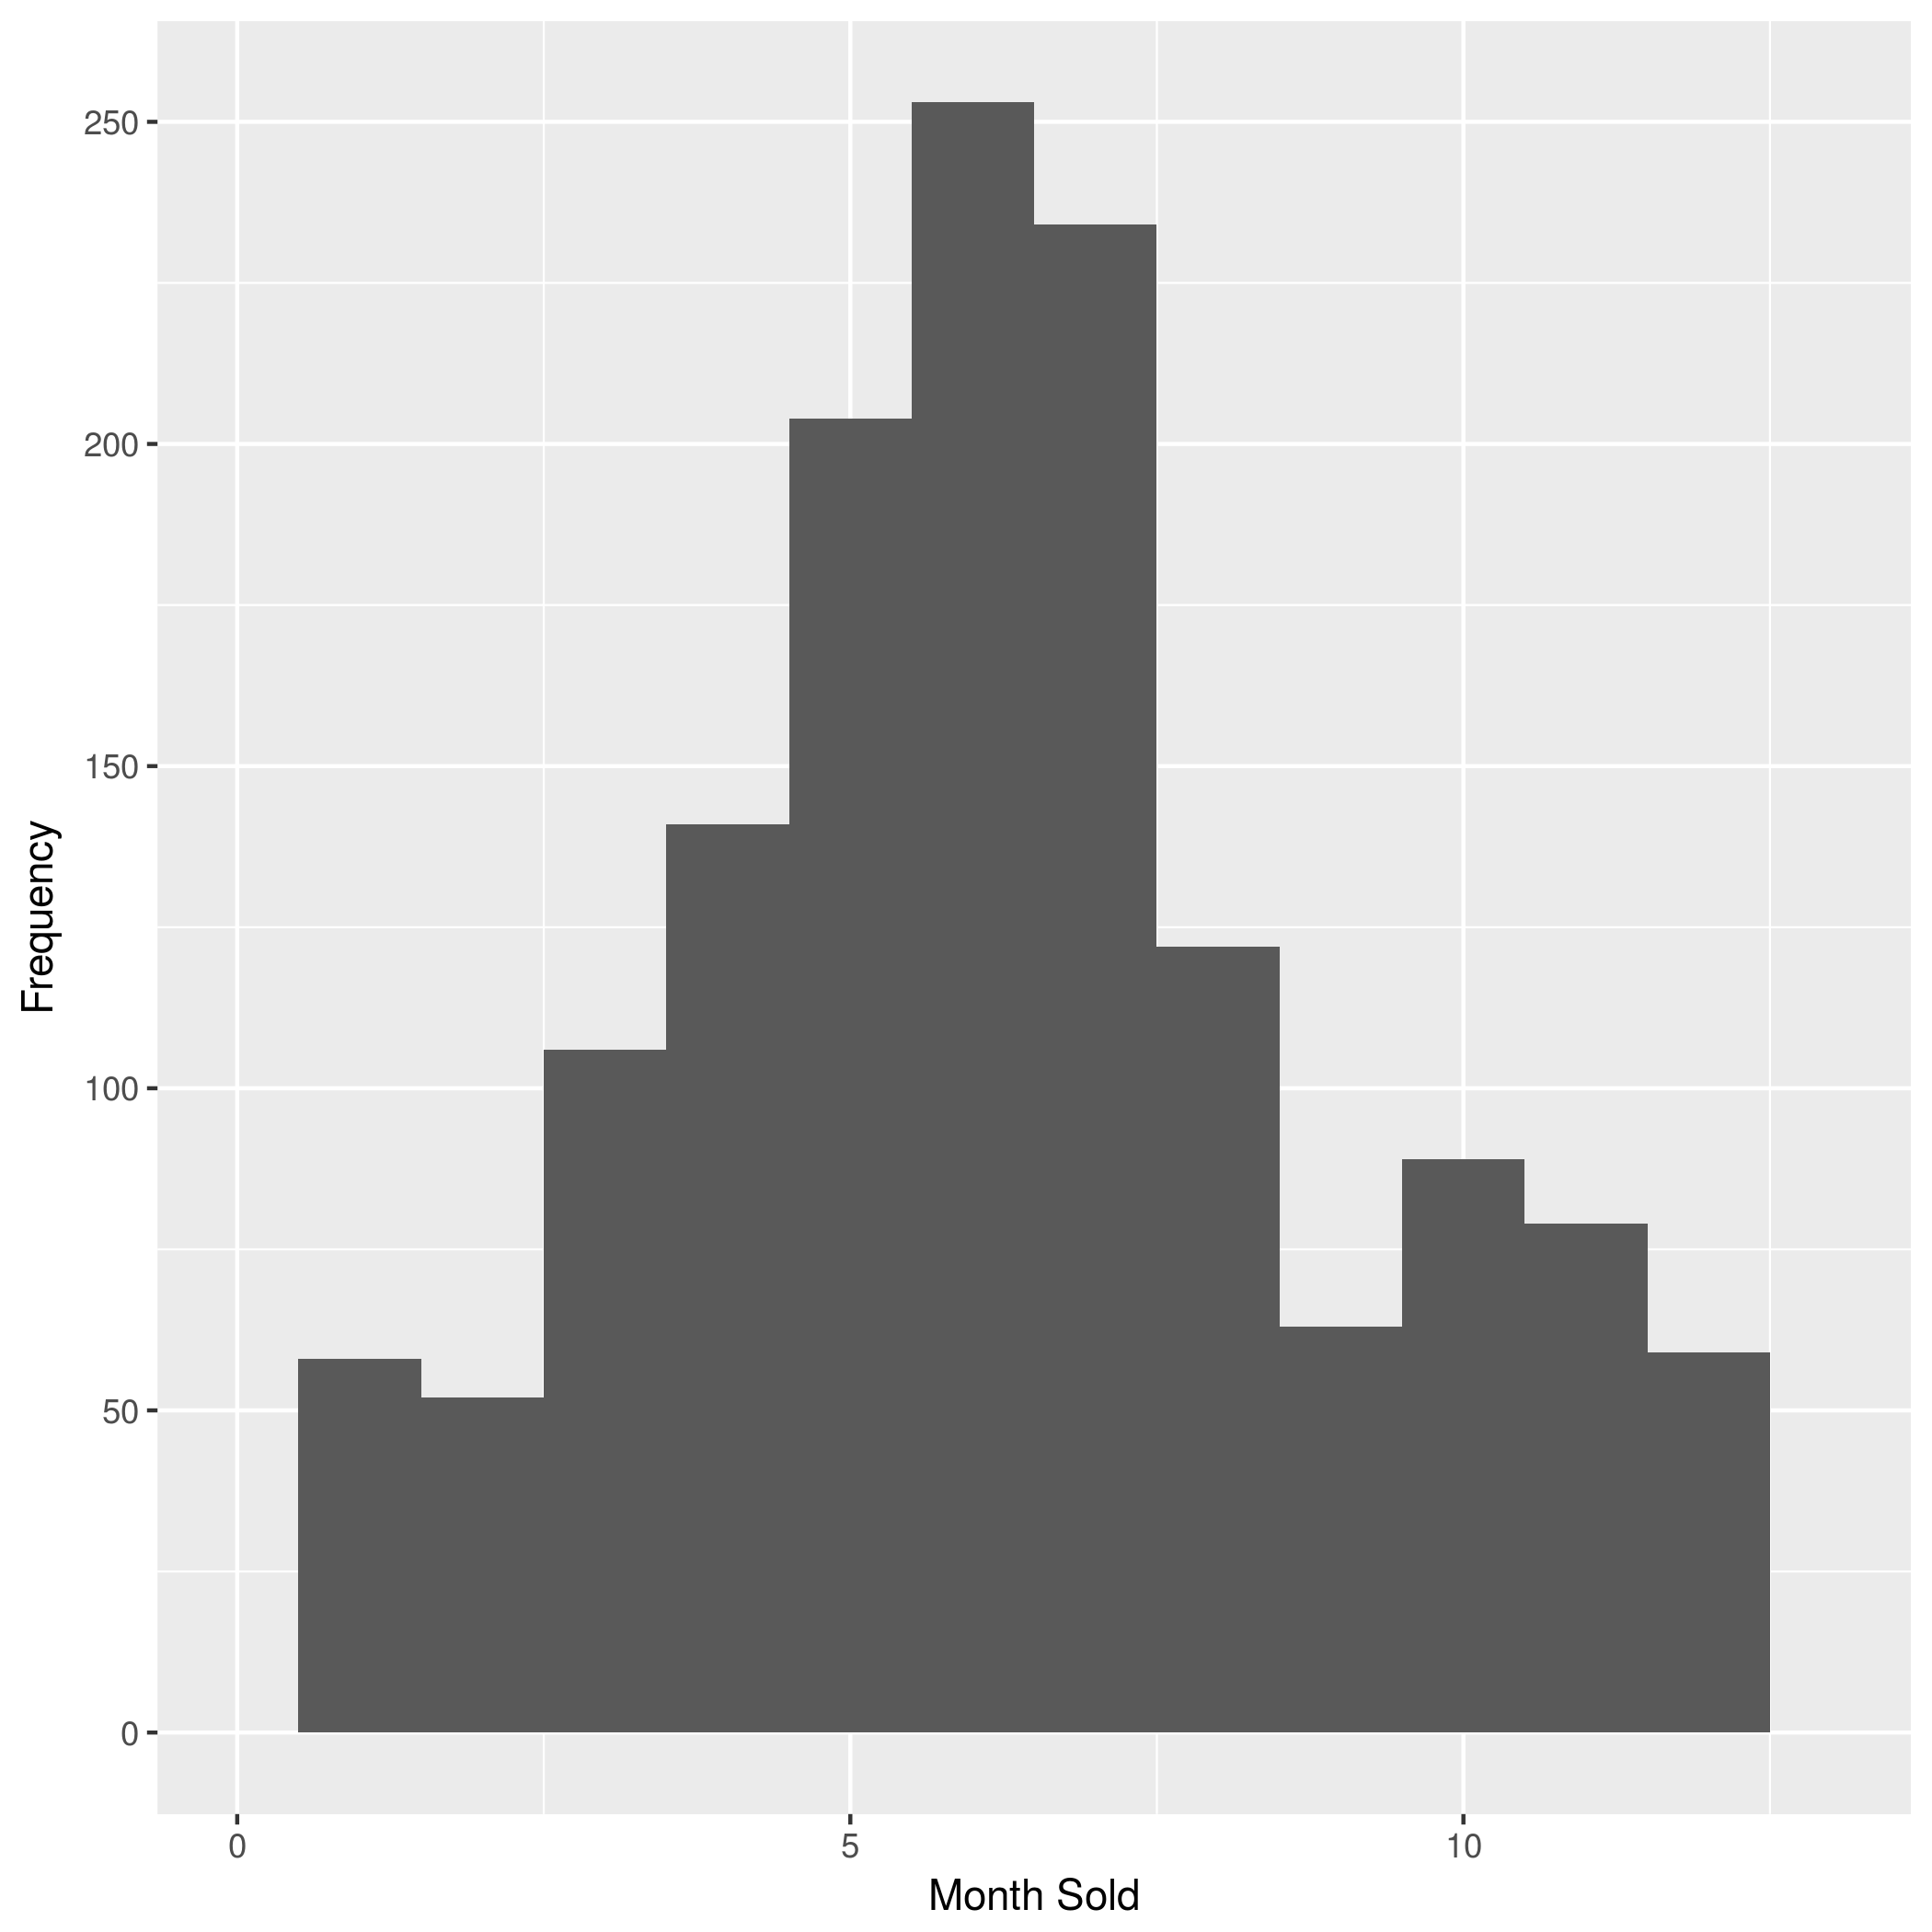
\includegraphics[scale = 0.60]{plot3.png}\\[1.0 cm]
\end{flushleft}
\begin{flushleft}
Looking at the histogram of mosold we see many more houses being sold near summer time so we create a boolean. Most of the time, when we are creating a boolean, it is because the individual levels are insignificant otherwise.

\centering
\section{Exploratory Data Analysis}
    \vspace*{0.5 cm}
    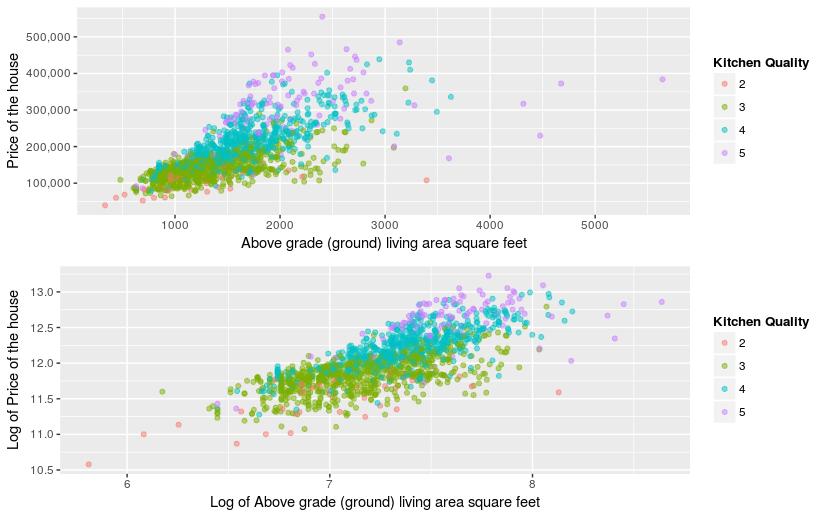
\includegraphics[scale = 0.75]{plot1.png}

\begin{flushleft}
We explore relationship between potential predictors with the response variable by plotting and calculating a correlation matrix. Some variables have a strong linear relationship with the sales price. In fact, two of the best predictors of house price -- kitchen quality and above grade (ground) living area square feet. In the top graph, we see that there is a fan-shape, which indicates homoscedasticity. This is why we considered to take the log of both the explanatory and response variable to solve this problem in our later transformations.

So, in the bottom plot, we see a fairly linear trend. As kitchen quality improves, the price of the house, on average, will also increase. Many of the houses fall within 3 or 4, which makes sense since it indicates the middle range. Furthermore, although obvious, as the square footage increases, the price of the house will also increase.
\end{flushleft}

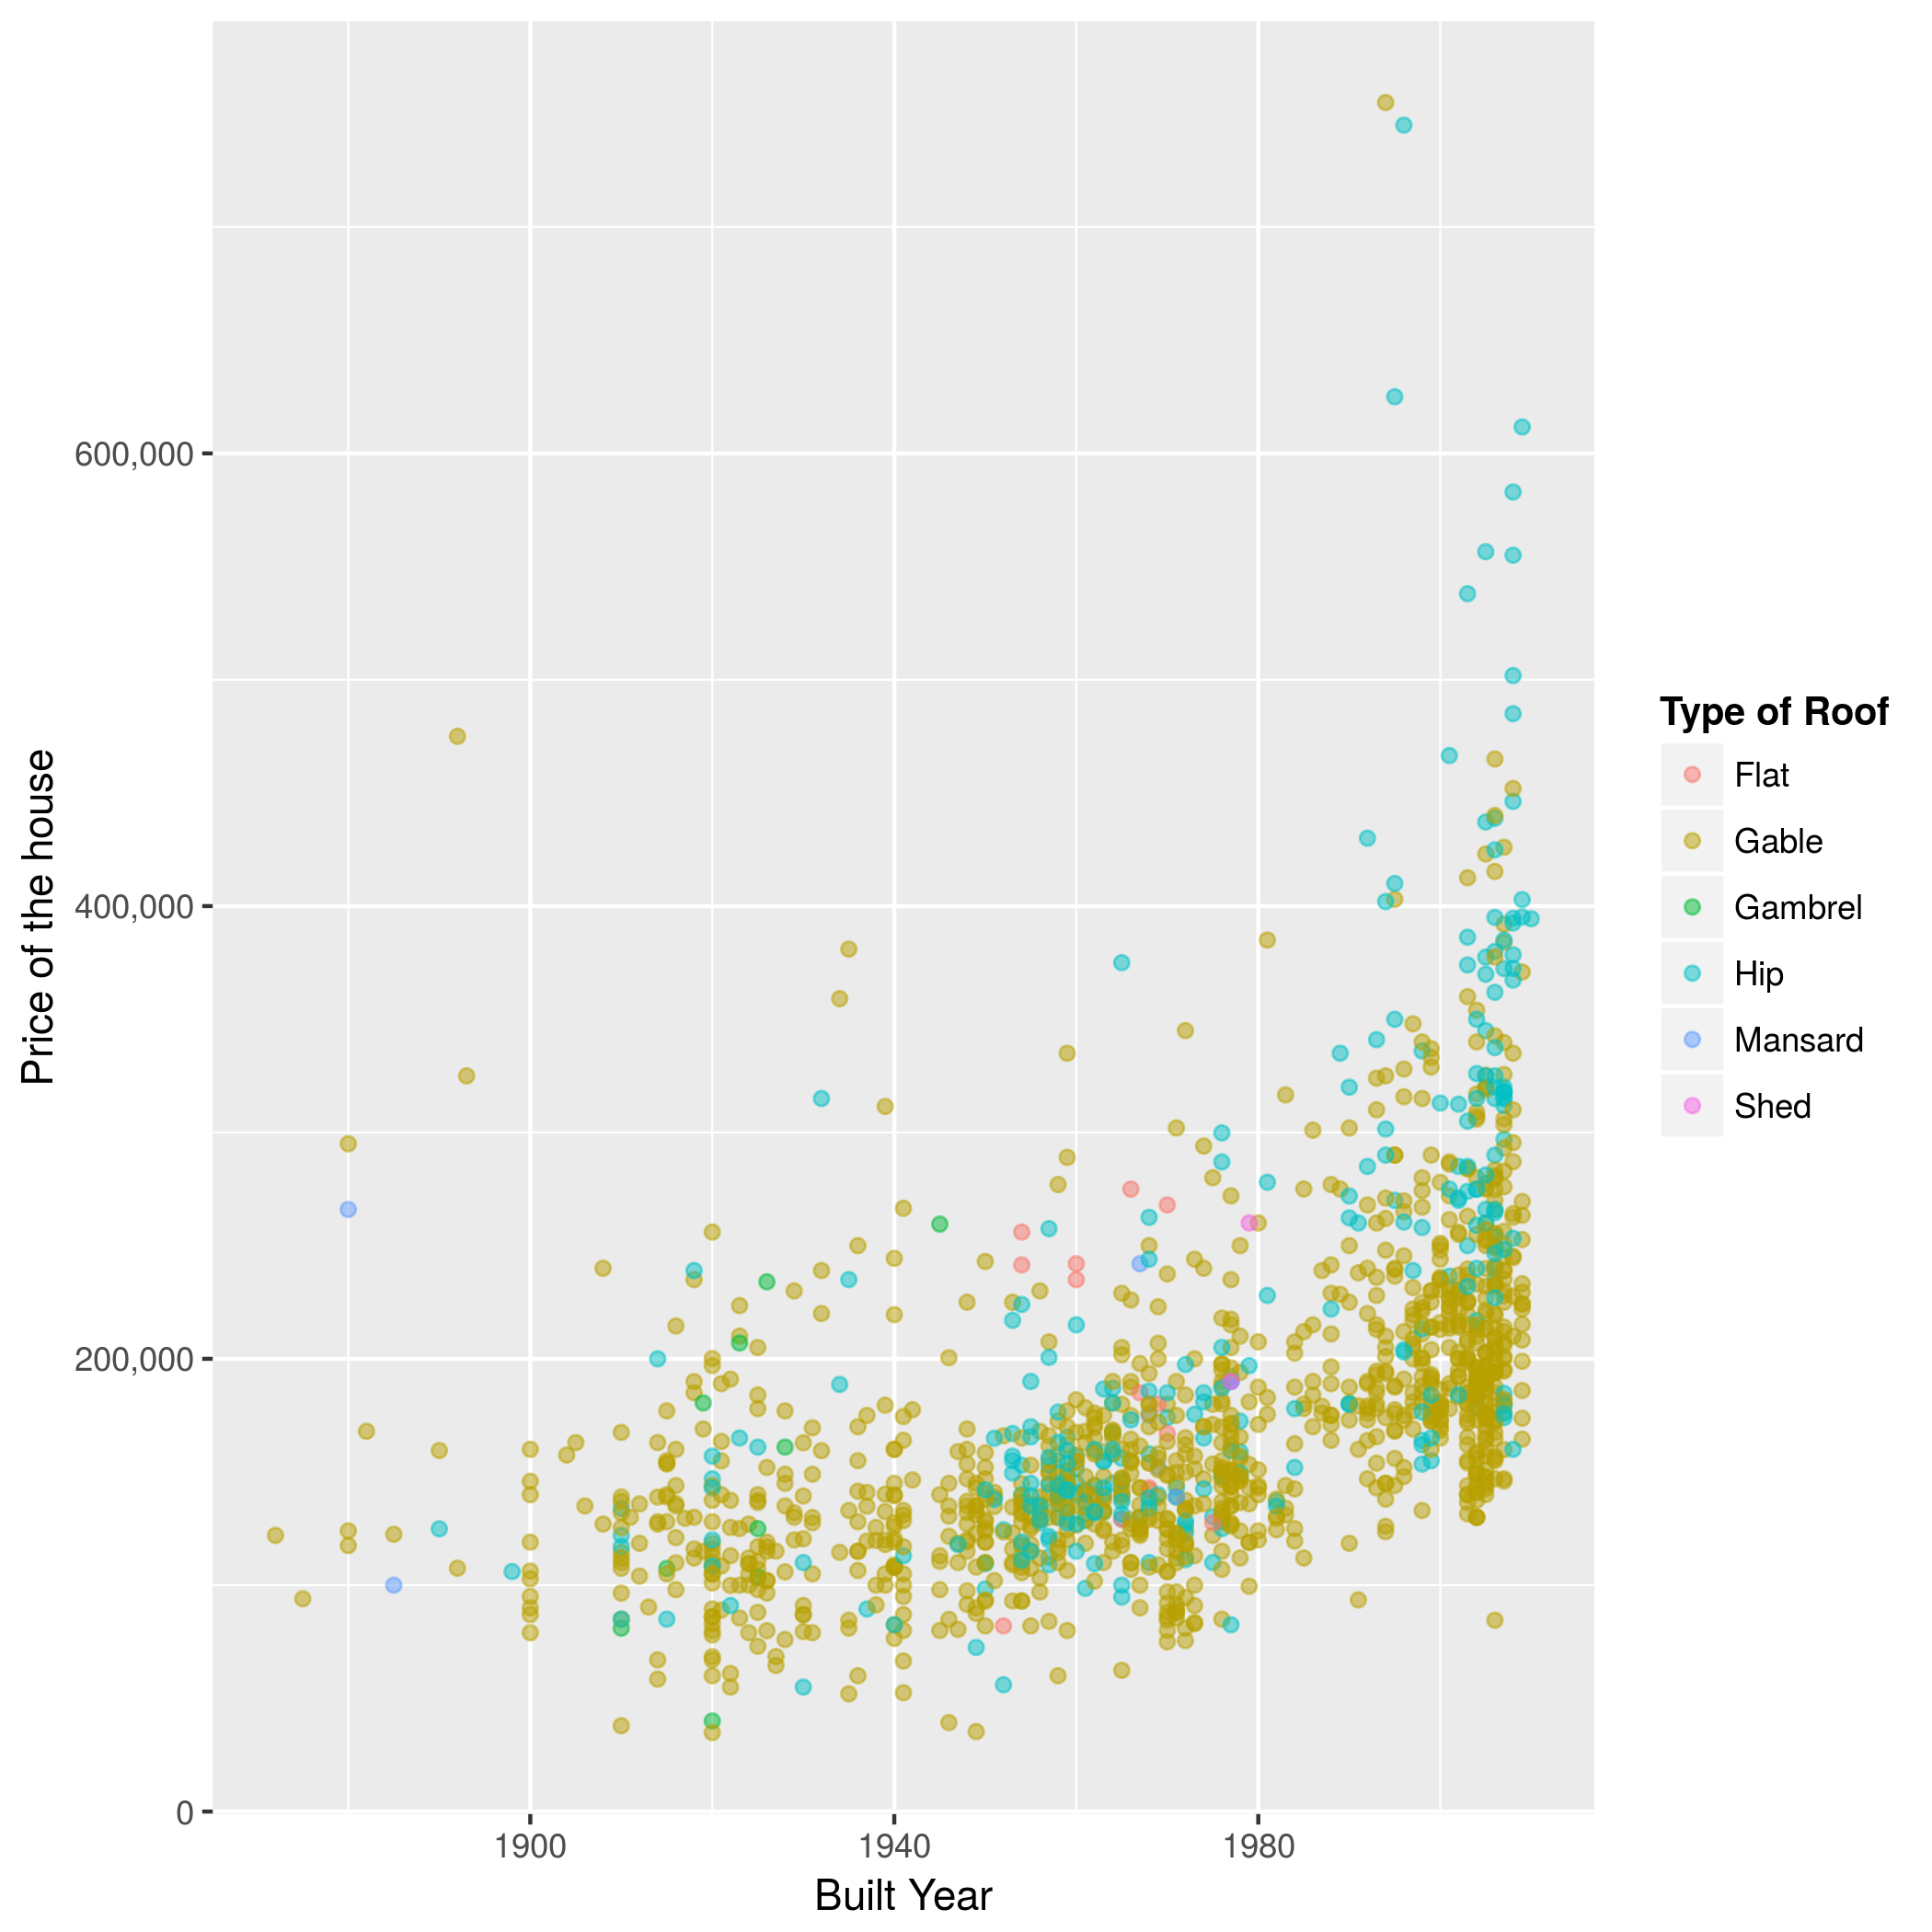
\includegraphics[scale = 0.40]{plot2.png}

\begin{flushleft}

This plot displays the price of houses over time, categorized by the type of roof. We can see that an overwhelming majority of houses are Gable houses. Hip houses are also somewhat common. In the 1960s, we see some Flat houses (in red). Throughout time, we see a general increase in the price of Hip houses over that of Gable houses. In particular, many of the extremely expensive houses are Hip ones. Most of  the houses are under \$ 200,000 but there seems to be an increase in the past years, which may just be due to inflation.
\end{flushleft}

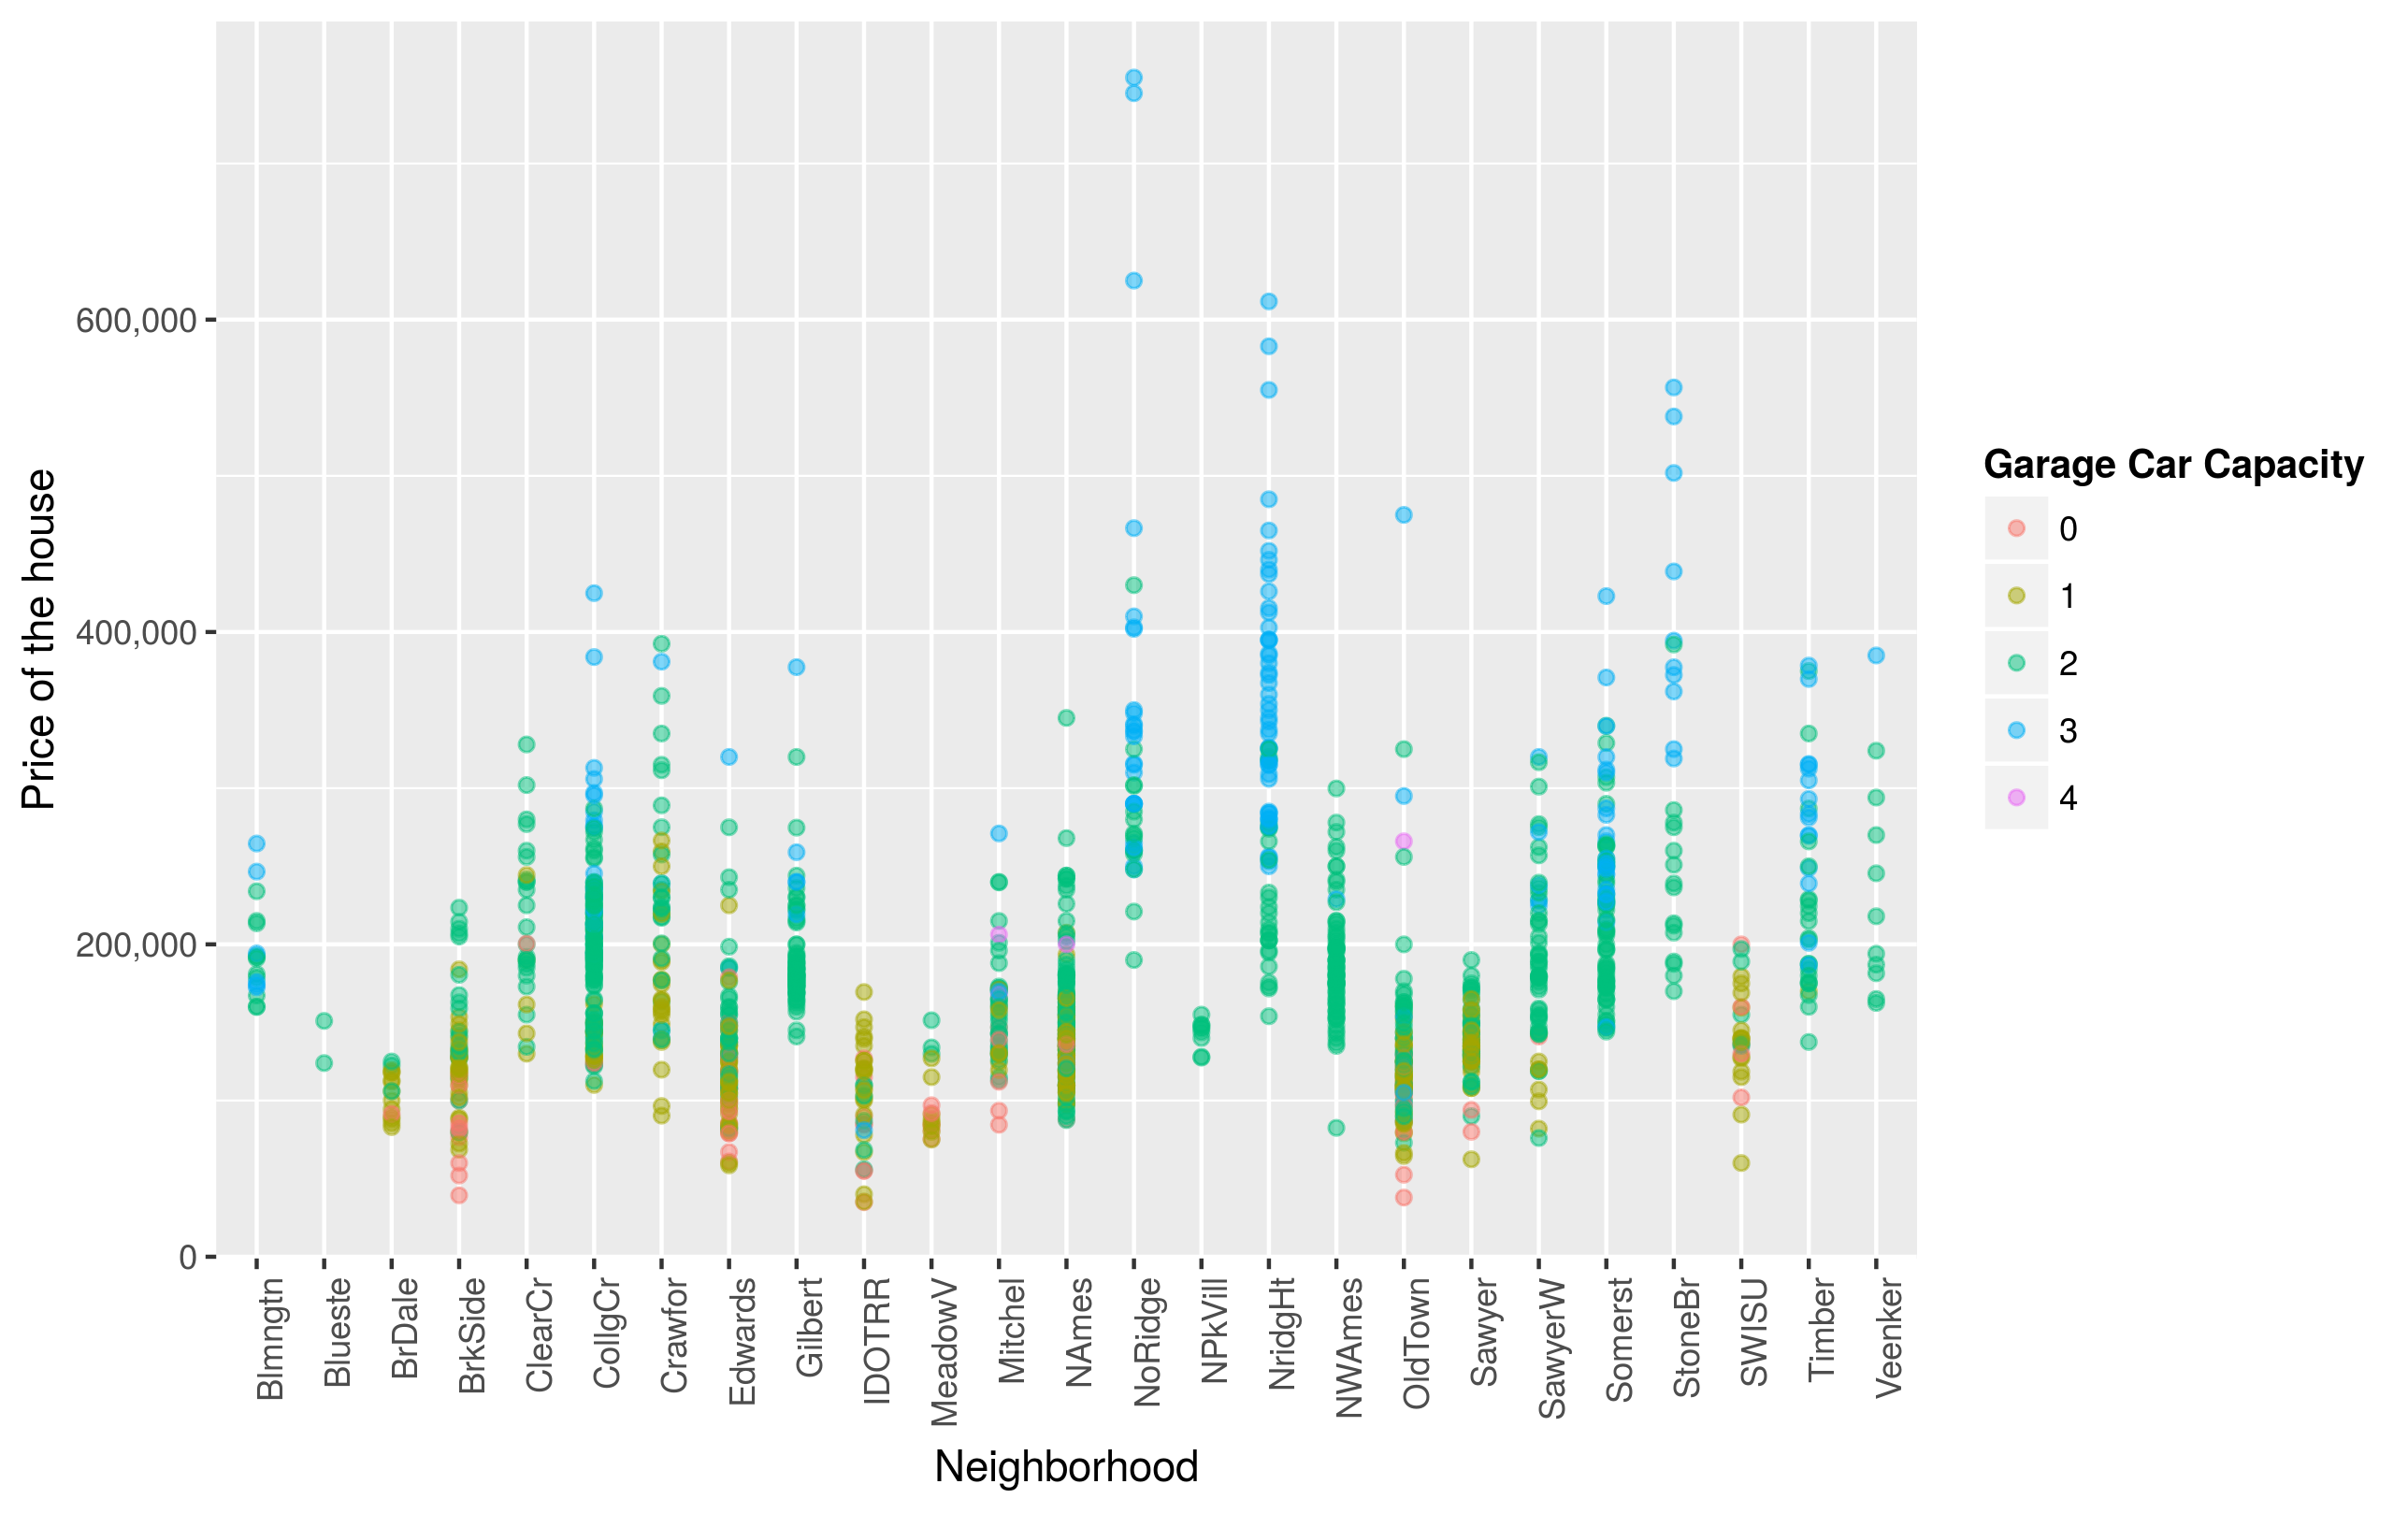
\includegraphics[scale = .6]{neighborhood.png}

\begin{flushleft}
Here, we see that neighborhood is definitely an important indicator of saleprice. Intuitively, some neighborhoods are much more expensive on average compared to other neighborhoods. The number of cars that can fit in the garage is also an important indicator of salesprice. Note that there are many other garage variables that will be affected as if the variable garagecars actually increases (meaning the garage gets extended).
\end{flushleft}

\centering
\section{Building the Model}
\begin{flushleft}
We perform a method that is similar to backwards selection (though manually). We start from the full model and remove insignificant variables one by one. The steps are as follows:
\end{flushleft}
\begin{enumerate}

\item Check the p-value and signifiance for a particlar variable.
\item (For Categorical) Use the table function to group the counts and/or hist function to make a quick histogram. 
\item (For Categorical) Use dplyr and group\_by to look at the median price for each category.
\item If the variable is numeric and significant, keep it. If the variable is categorical and all levels are significant, keep it. If only some levels are significant then try to bin the factors into smaller number of levels to try and make them statistically significant. If nothing can be done, then remove the variable.
\item Repeat steps 1 through 4 for the rest of the variables. Each time we remove a variable, we re-run the lm model to check if the Adjusted R Squared changed significantly or not. If it decreased, we may add the variable back.
\item When we finish going through all the variables, there will be about 30 ones left to consider.
\item Stop when every single variable becomes statistically signifcant under an $\alpha$ level of 0.05. Confirm results with variable selection via LASSO.
\end{enumerate}

\subsection{LASSO Results}
\begin{flushleft}

We performed LASSO on the 30 variables obtained from backwards selection. LASSO only turned the Neighborhoods Gilbert, NpkVill, NWAmes, Sawyer, SawyerW along with the variables bsmtunfsf and bedroomabvgr to zero. Many of the neighborhoods are significant so we keep the non-significant ones since it doesn't make sense to remove them. We attempted to remove bsmtunsf and bedroomabvgr but we found that they reduced our R squared so we kept them as well. Overall, LASSO confirmed the significance of the predictors that we picked.
\end{flushleft}
\subsection{Notes}
\begin{itemize}
\item The variable grlivarea is equal to the sum of the variables 1stflrsf, 2ndflrsf, and lowqualfinsf. At first, we tried having all three of them and deleting grlivarea however we found that having just grlivarea performed better.
\item We modified the reference levels for the categorical variables to the most logical and/or most common level.
\item We changed ordered factors to numeric, e.g. None, Po, Fa, TA, Gd, Ex 
\item If two variables are obviously correlated with each other, we choose the variable that has a higher correlation with sales price.
\item After processing the variables, everything becomes numeric. The only categorical variable left is Neighborhood.
\end{itemize}

After following the process stated above, there are 30 variables left:
\begin{center}
\begin{tabular}{|c|c|c|}
\hline

lotarea & bsmtexposure   &  garagetype \\ neighborhood &  bsmtfinsf1 &    garagecars \\
  condition1  & bsmtfinsf2    & wooddecksf \\
   condition2 &   bsmtunfsf    &   poolarea  \\
   housestyle &   heatingqc & salecondition \\
   overallqual &   grlivarea    & saleprice \\
   overallcond & bedroomabvgr   &     remodel \\
      roofmatl & kitchenabvgr & soldminusbuilt \\
    masvnrtype & kitchenqual  &   summertime \\
   masvnrarea &  functional &       saletype \\  \hline 

\end{tabular}
\end{center}
\begin{samepage}
\centering
\section{Multicollinearity}
\begin{flushleft}When selecting variables, we noticed some variables refer to the same feature of house. For example, totrmsabvgrd (total rooms above grade) and grlivarea (Above grade living area square feet) are obviously correlated. In these cases, we choose the variable with higher correlation with salesprice since it explains salesprice better. 

After the variables are selected, we  use the variance inflation factors(VIF) to test the multicollinearity on the whole model. A VIF greater than 10 indicates significant multicollinearity. The VIF computed from our constructed models are lower than the threshold so these models pass the multicollinearity test successfully.

Some variables have exact multicollinearity, such as grlivarea with 1stflrsf, 2ndflrsf, and lowqualfinsf. We decide to keep grlivarea after experimenting with both of them because we get better results with just grlivarea. 

When computing the VIF, we remove the categorical variable neighborhood.
\end{flushleft}
\centering
    \vspace*{0.5 cm}
    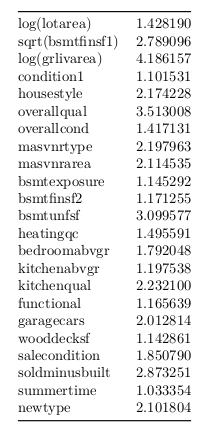
\includegraphics[scale = .5]{vif.png}\\[1.0 cm]	


\end{samepage}
\centering
\section{Transformations}
\begin{flushleft}

As for now, we have 30 significant variables, 6 of them has a correlation with sale price that is greater than 0.5. We wish to check the normality of numerical variables so that we will have a better understanding what transformation we need or if we need transformation on our variables. In these 6 variables as well as salesprice, only salesprice and grlivarea are continuous. In the below Q-Q plots, the first plots the quantiles of the standardized grlivarea values against those of a normal distribution. It’s obvious that it has two big tails that are not on the line. We decided that a log transformation is necessary for grlivarea. After taking a log transformation on grlivarea, most of points are nicely placed around the line in its Q-Q plot. Salesprice, on the other hand, is not normal distributed, so again we take a log on salesprice. The new plots look good and no longer have a curved shape.

\end{flushleft}
\centering
    \vspace*{0.5 cm}
    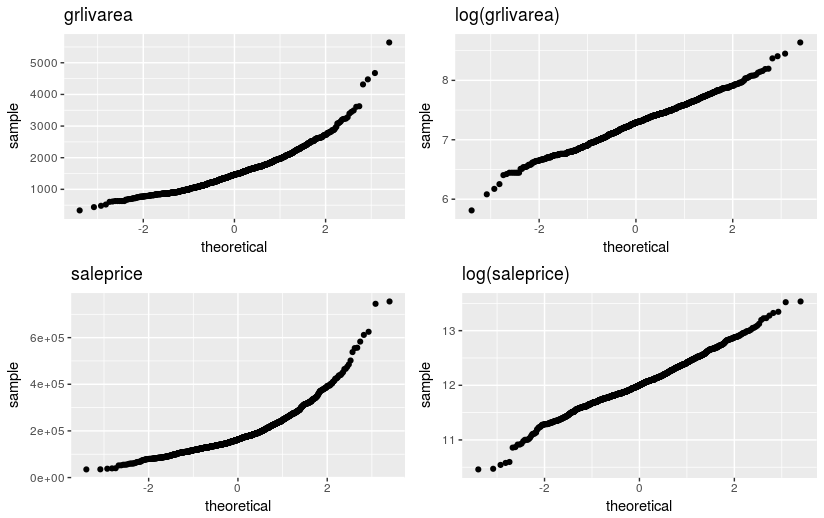
\includegraphics[scale = .5]{qq.png}\\[1.0 cm]	
\begin{flushleft}

As a result, the model now has 6 variables and we take log transformation of both response variable and one predictor variable. In this new model, checking p-values, we realized that one of them (exterqual) becomes insignificant. So we further delete this variable and now we have a model with 5 variables.

For the other variables, after some experimentation, we also take the log of lotarea and the square root of bsmtfinsf1 in our final model. 

For clarification, we work with two seperate models. One model contains only the \textit{best} predictors (correlation greater than 0.5). After transforming more variables, we found 5 variables from the full model to no longer be significant. The \textit{full} model contains statistically significant variables and ends up to be 23 variables, with one of them as categorical (Neighborhood). 
\end{flushleft}
\section{Normality and Homoscedascity}
\begin{flushleft}

Our linear regression are based on the assumption of normal errors. The residuals can be assessed for normality using the Q-Q plot below. This compares the residuals to “ideal” normal observations. After transforming the data and deleting influential points, we hope that the errors are normally distributed.
The below residual Q-Q plot shows that more than half of the points are located around the line. Further, Kolmogorov-Smirnov test gives us a p-value of 0.05036, which is not bad. So we believe our model passed the normality test.

We see that the assumption of homoscedascity is met. In the residual plot below, we see that there is no clustering or any systematic pattern. We formally test non-constance variance with the Breusch-Pagan test. Because we get a very low p-value of 0.00249, we are confident there is no heteroscedascity occurring.
\end{flushleft}
\centering
    \vspace*{0.5 cm}
    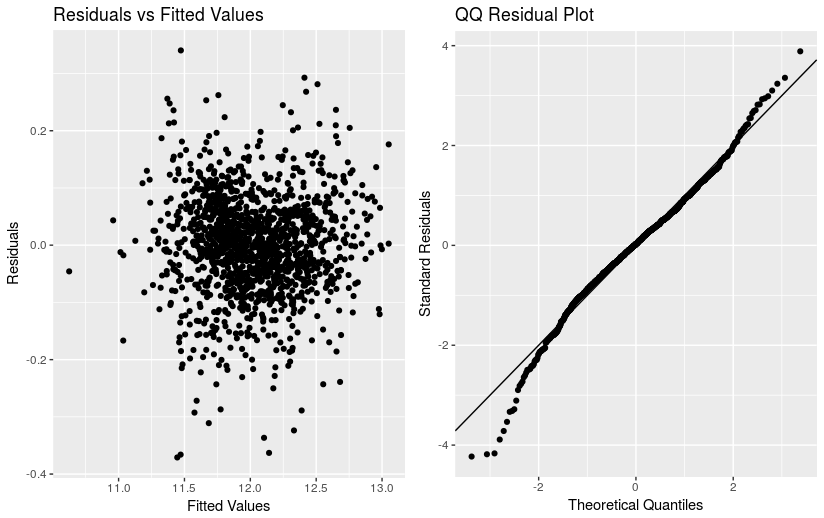
\includegraphics[scale = .5]{res.png}\\[1.0 cm]	
\begin{flushleft}
\centering
\section{Point Diagnostics}
\begin{flushleft}
First, let's distinguish between the three similar, but different terms of leverage points, influential points, and outliers.
\end{flushleft}
\subsection{Leverage Points}
\begin{flushleft}

A point has \textbf{high leverage} if it has a high \textit{hat value}. The hat values are the diagonals of the hat matrix: $H = X(X^{T}X)^{-1}X^{T}$. Another way to express this idea is to say that the x values are "extreme". A common rule of thumb is to say that a point has high leverage if
$h_{ii} > \frac{2p}{n}$. p is the number of predictors, or 30. n is the number of observations, or 1460. This makes our cut-off point 0.04. As we see in the graph below, all of the green points are high leverage points. There are a total of 98 high leverage points according to this threshold. Interestingly, there are two values with very high leverage points with hat values greater than 0.5. These are Observations 600 and 957.
\end{flushleft}
\centering
    \vspace*{0.5 cm}
    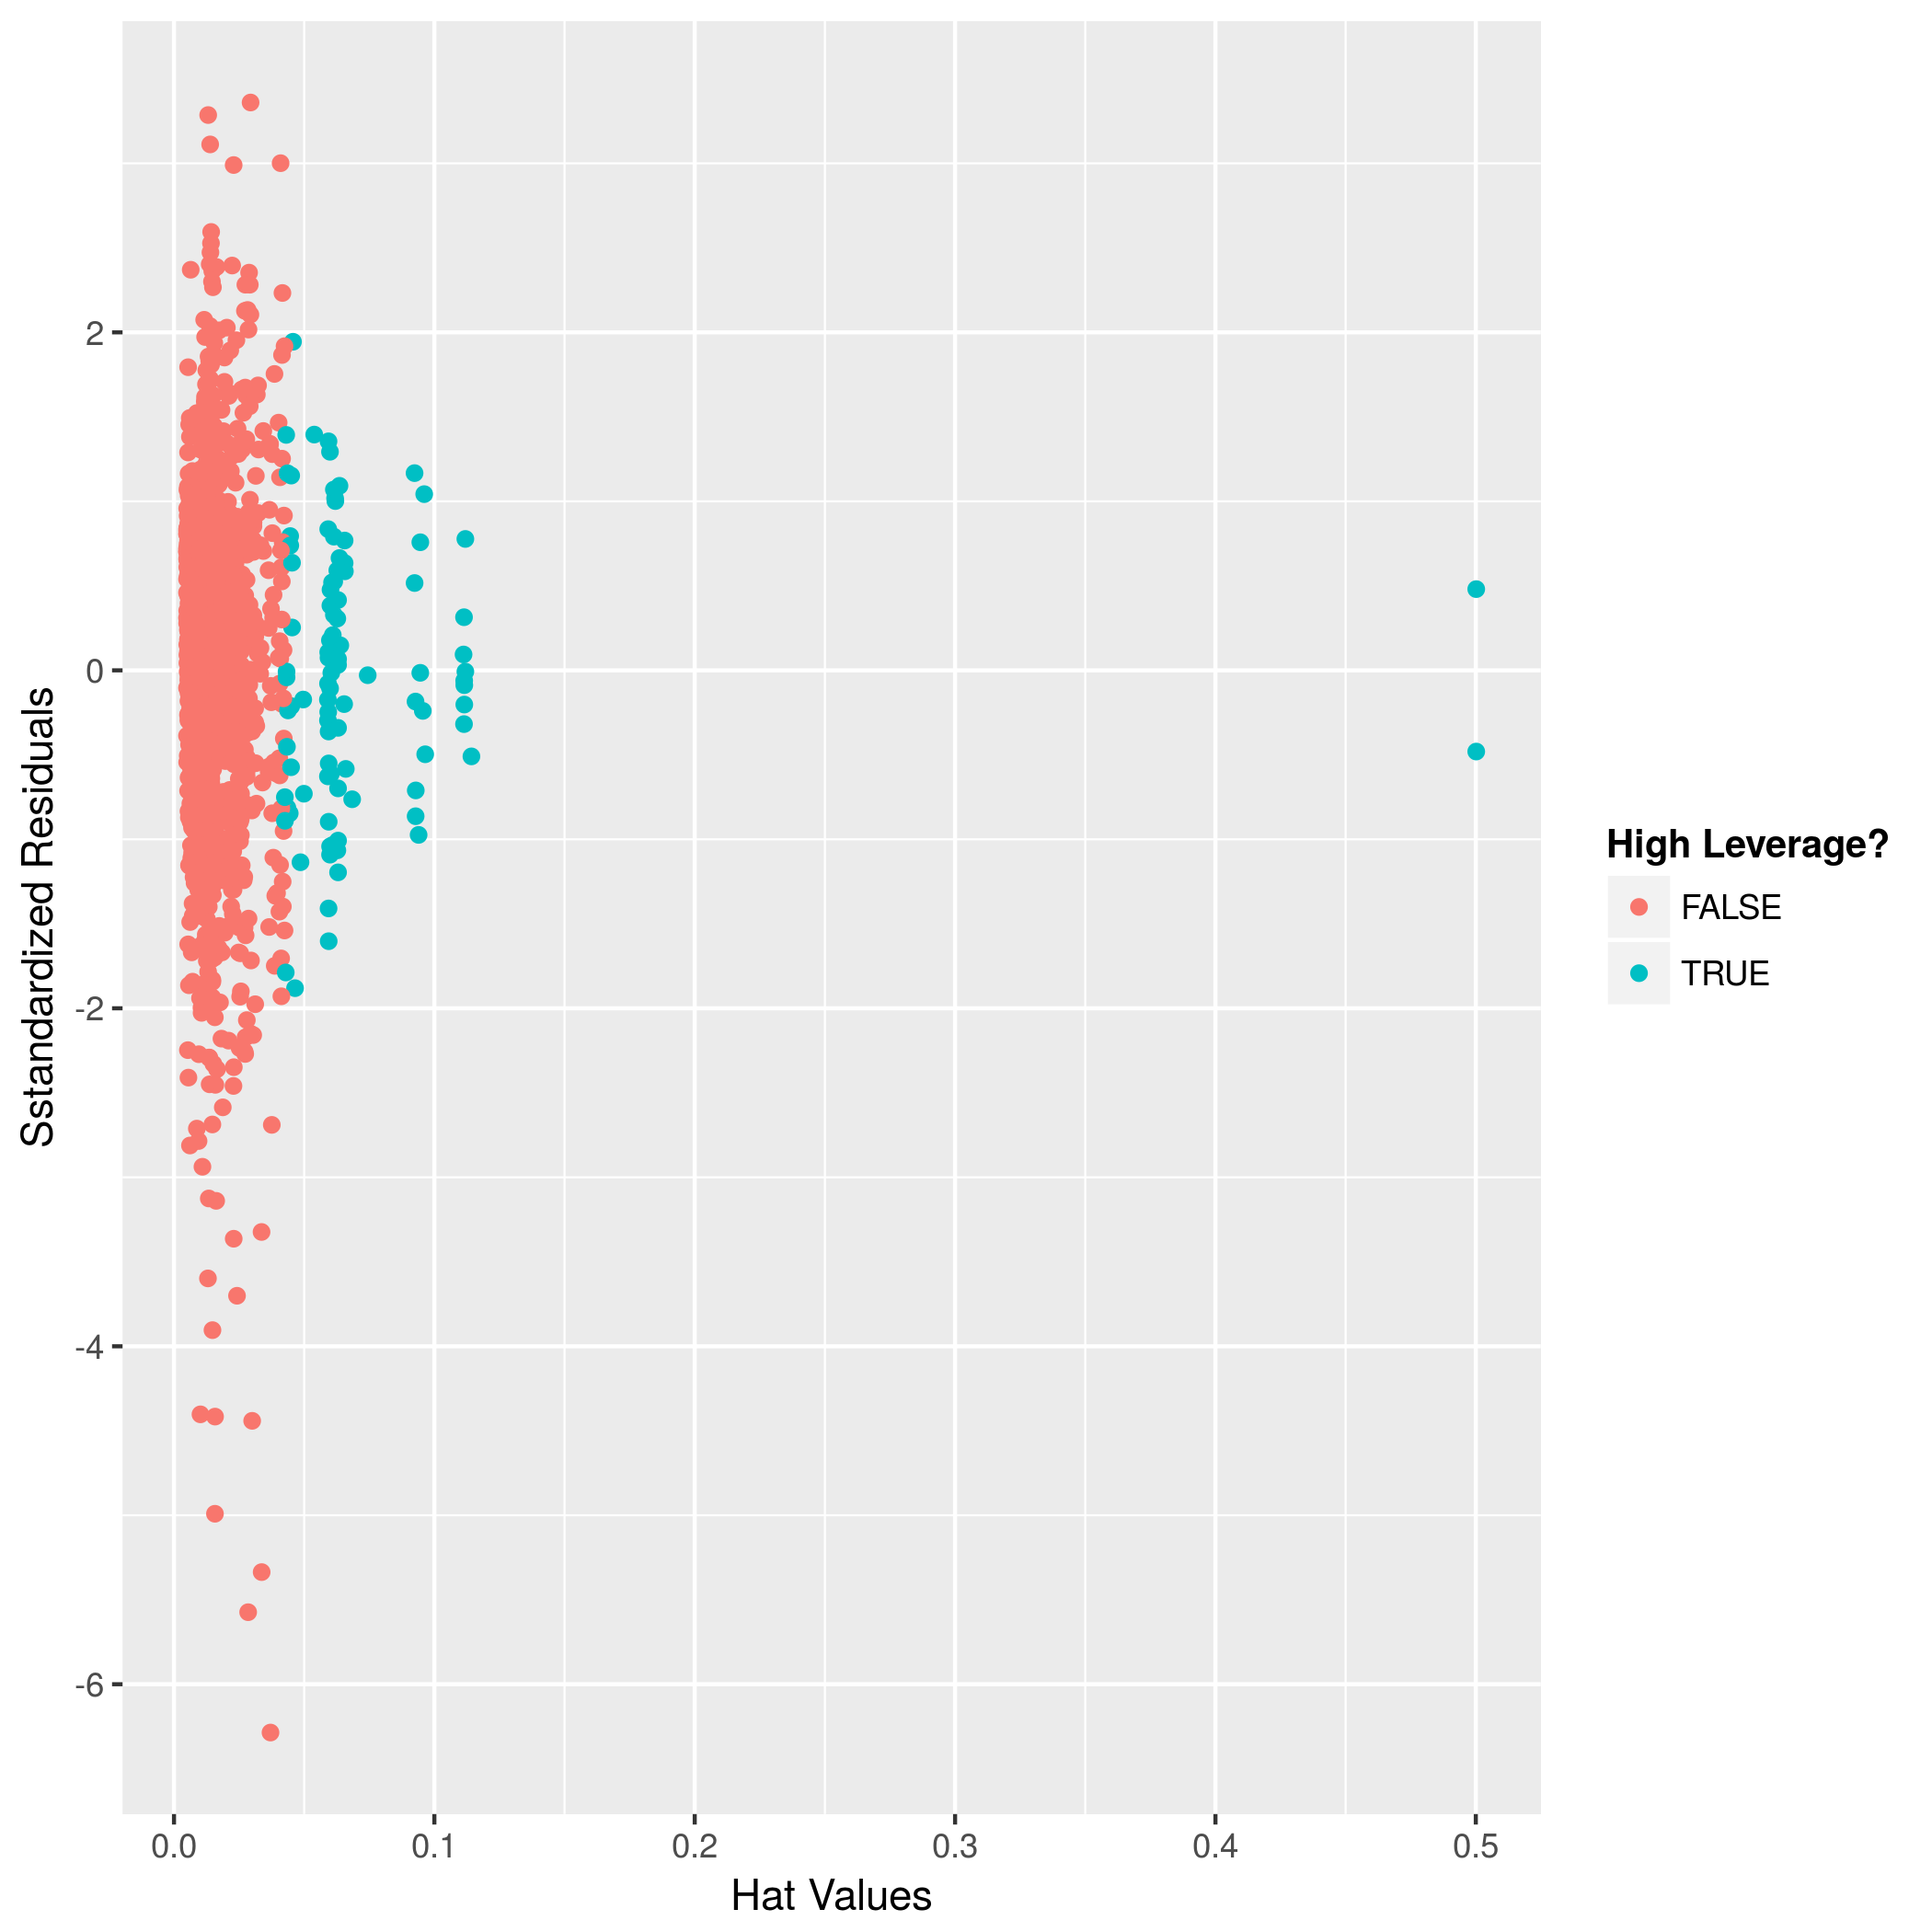
\includegraphics[scale = .40]{leverage.png}\\[1.0 cm]	
    
\begin{flushleft}
\subsection{Influential Points}

A point has \textbf{high influence} if its presence will have a distorting effect on the estimation of the parameters. We will use a rule of thumb and say that a point is influential if $DFFITS_{i} > \sqrt{\frac{2p}{n}}$. In the plot below, we see the green high influential points in both the positive and negative direction.

\end{flushleft}

\centering
    \vspace*{0.5 cm}
    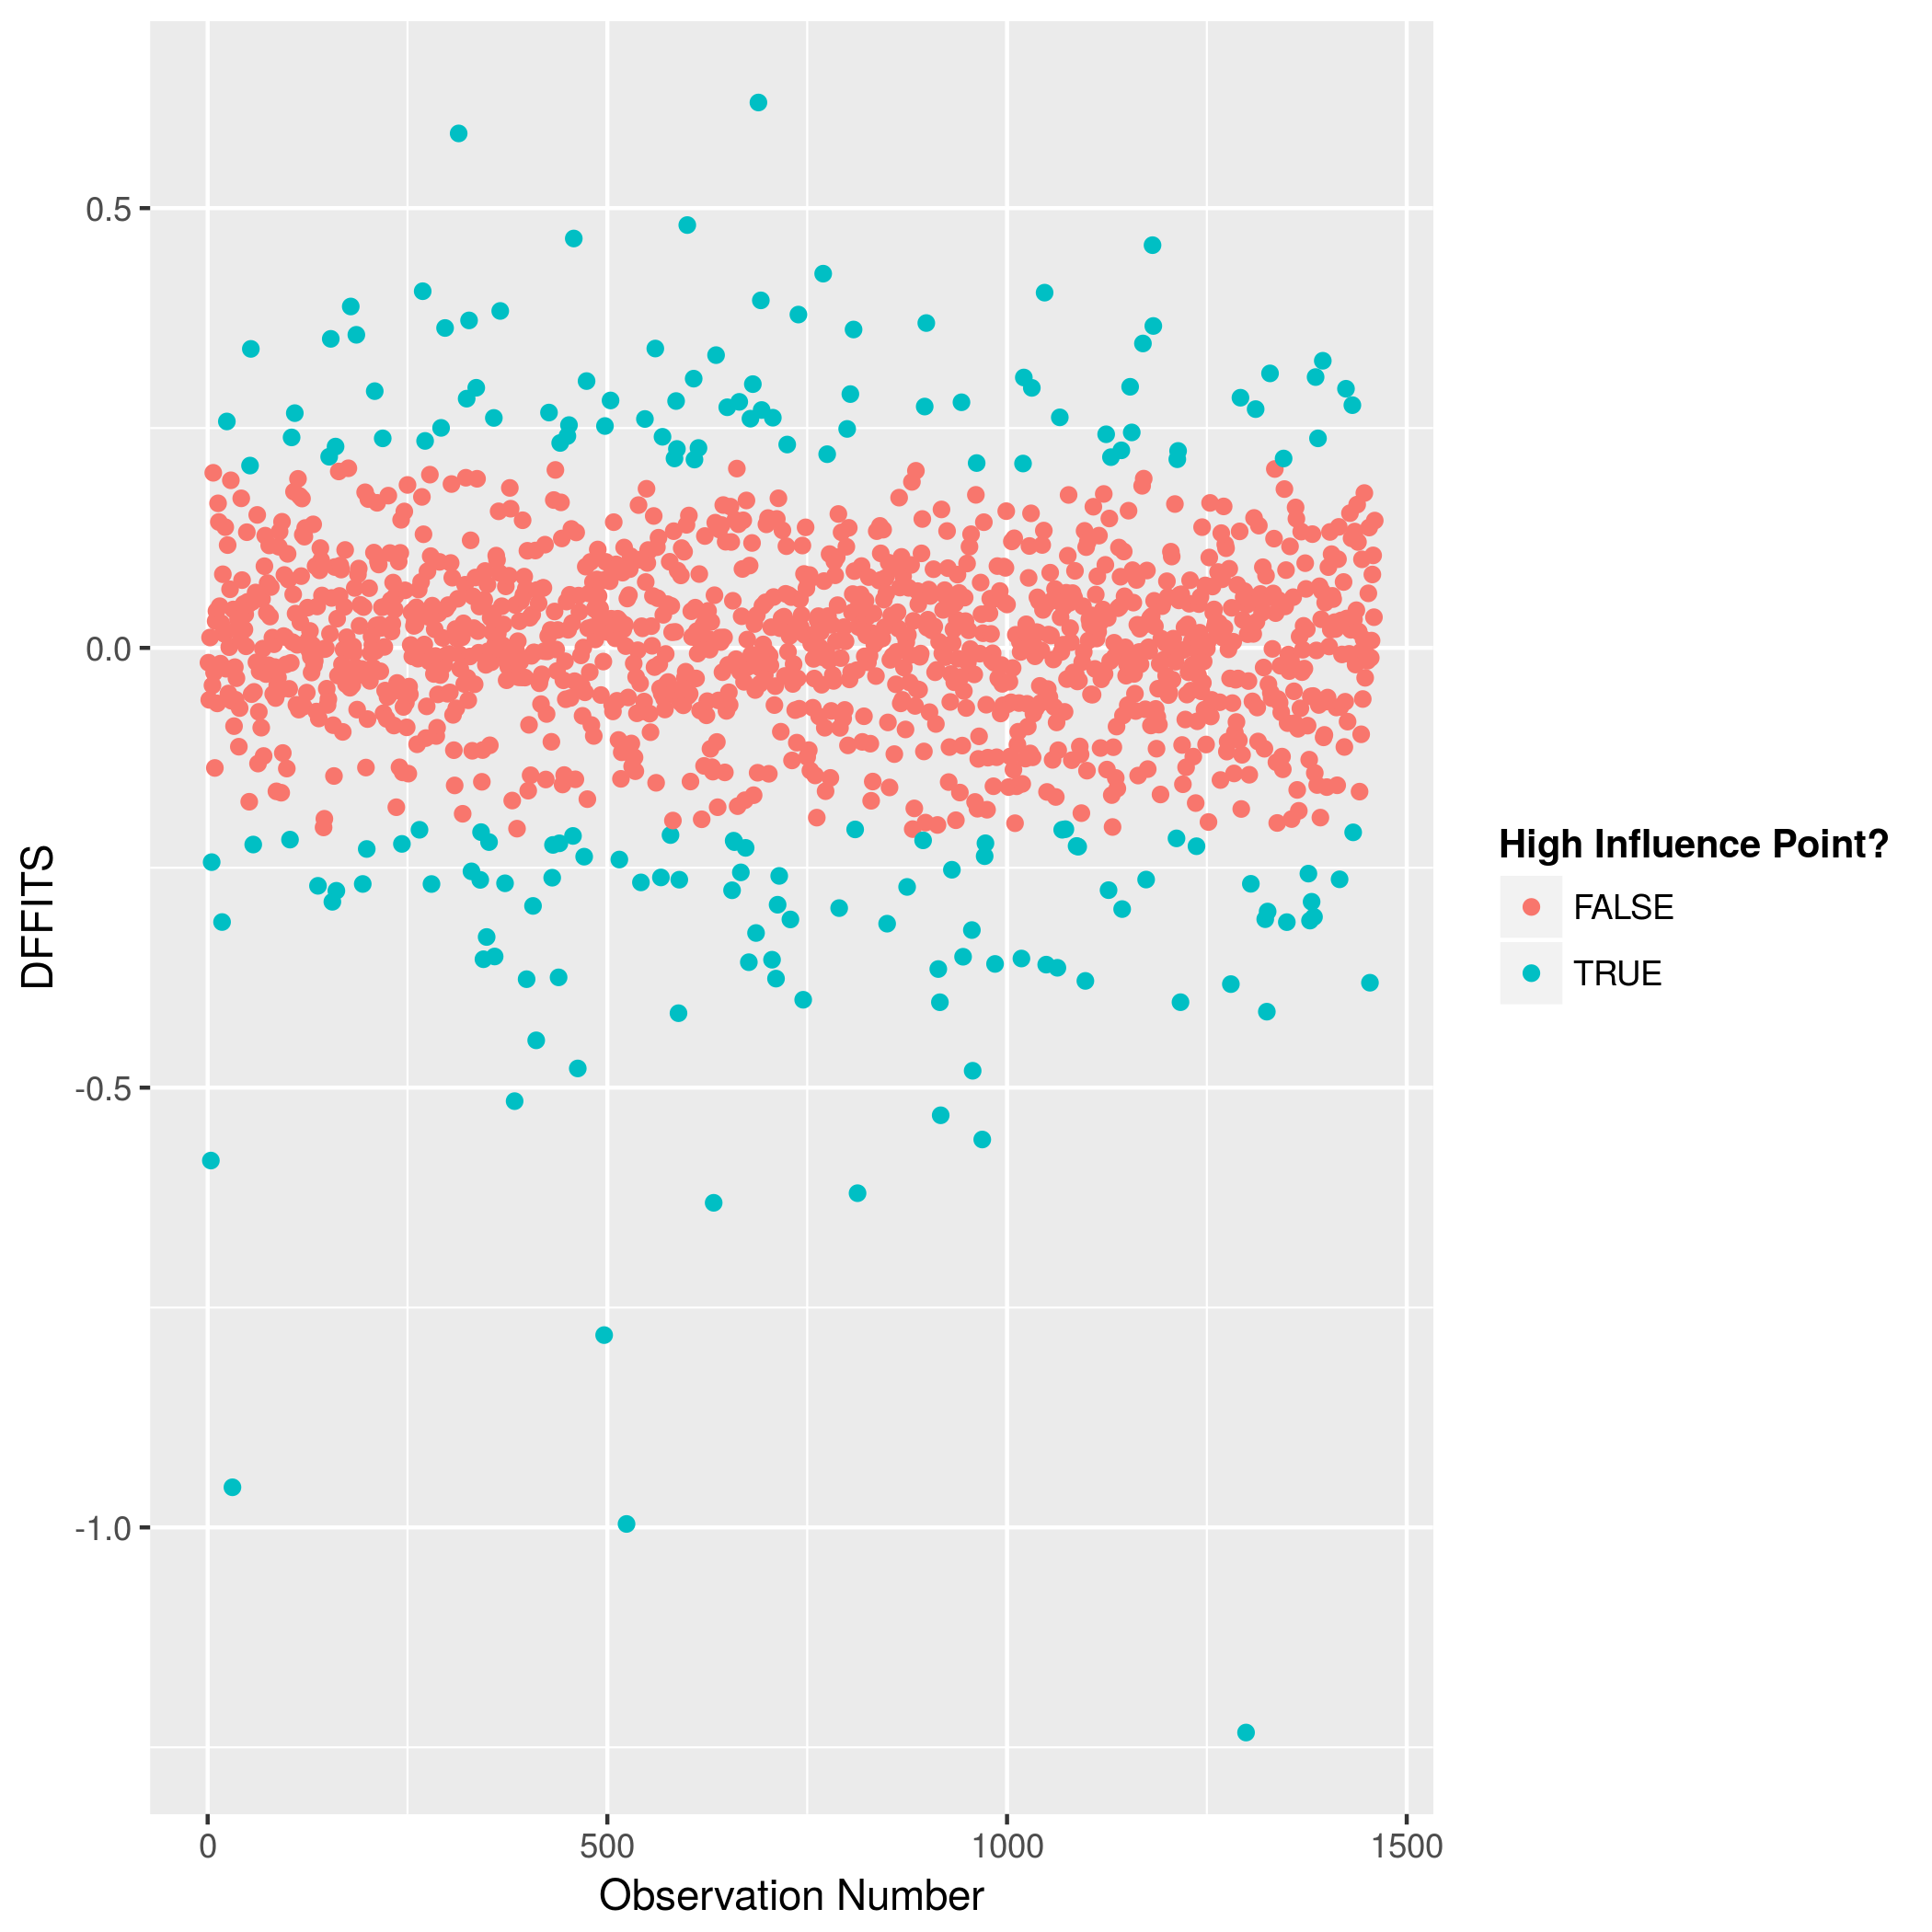
\includegraphics[scale = .40]{influence.png}\\[1.0 cm]	

\begin{flushleft}

\subsection{Outliers}
An observation i is an \textbf{outlier} if the residual $e_{i}$ is large. To determine whether an observation is an outlier, we will use the function ols\_dffits\_plot from the library olsrr. It is similar to what we did with influential points. It categorizes an outlier if it has a DFFIT greater than the threshold of 0.28. Note that it is more strict than  our high influence threshold. So all of the points outside the range of the red lines are classified as outliers.

\end{flushleft}

\centering
    \vspace*{0.5 cm}
    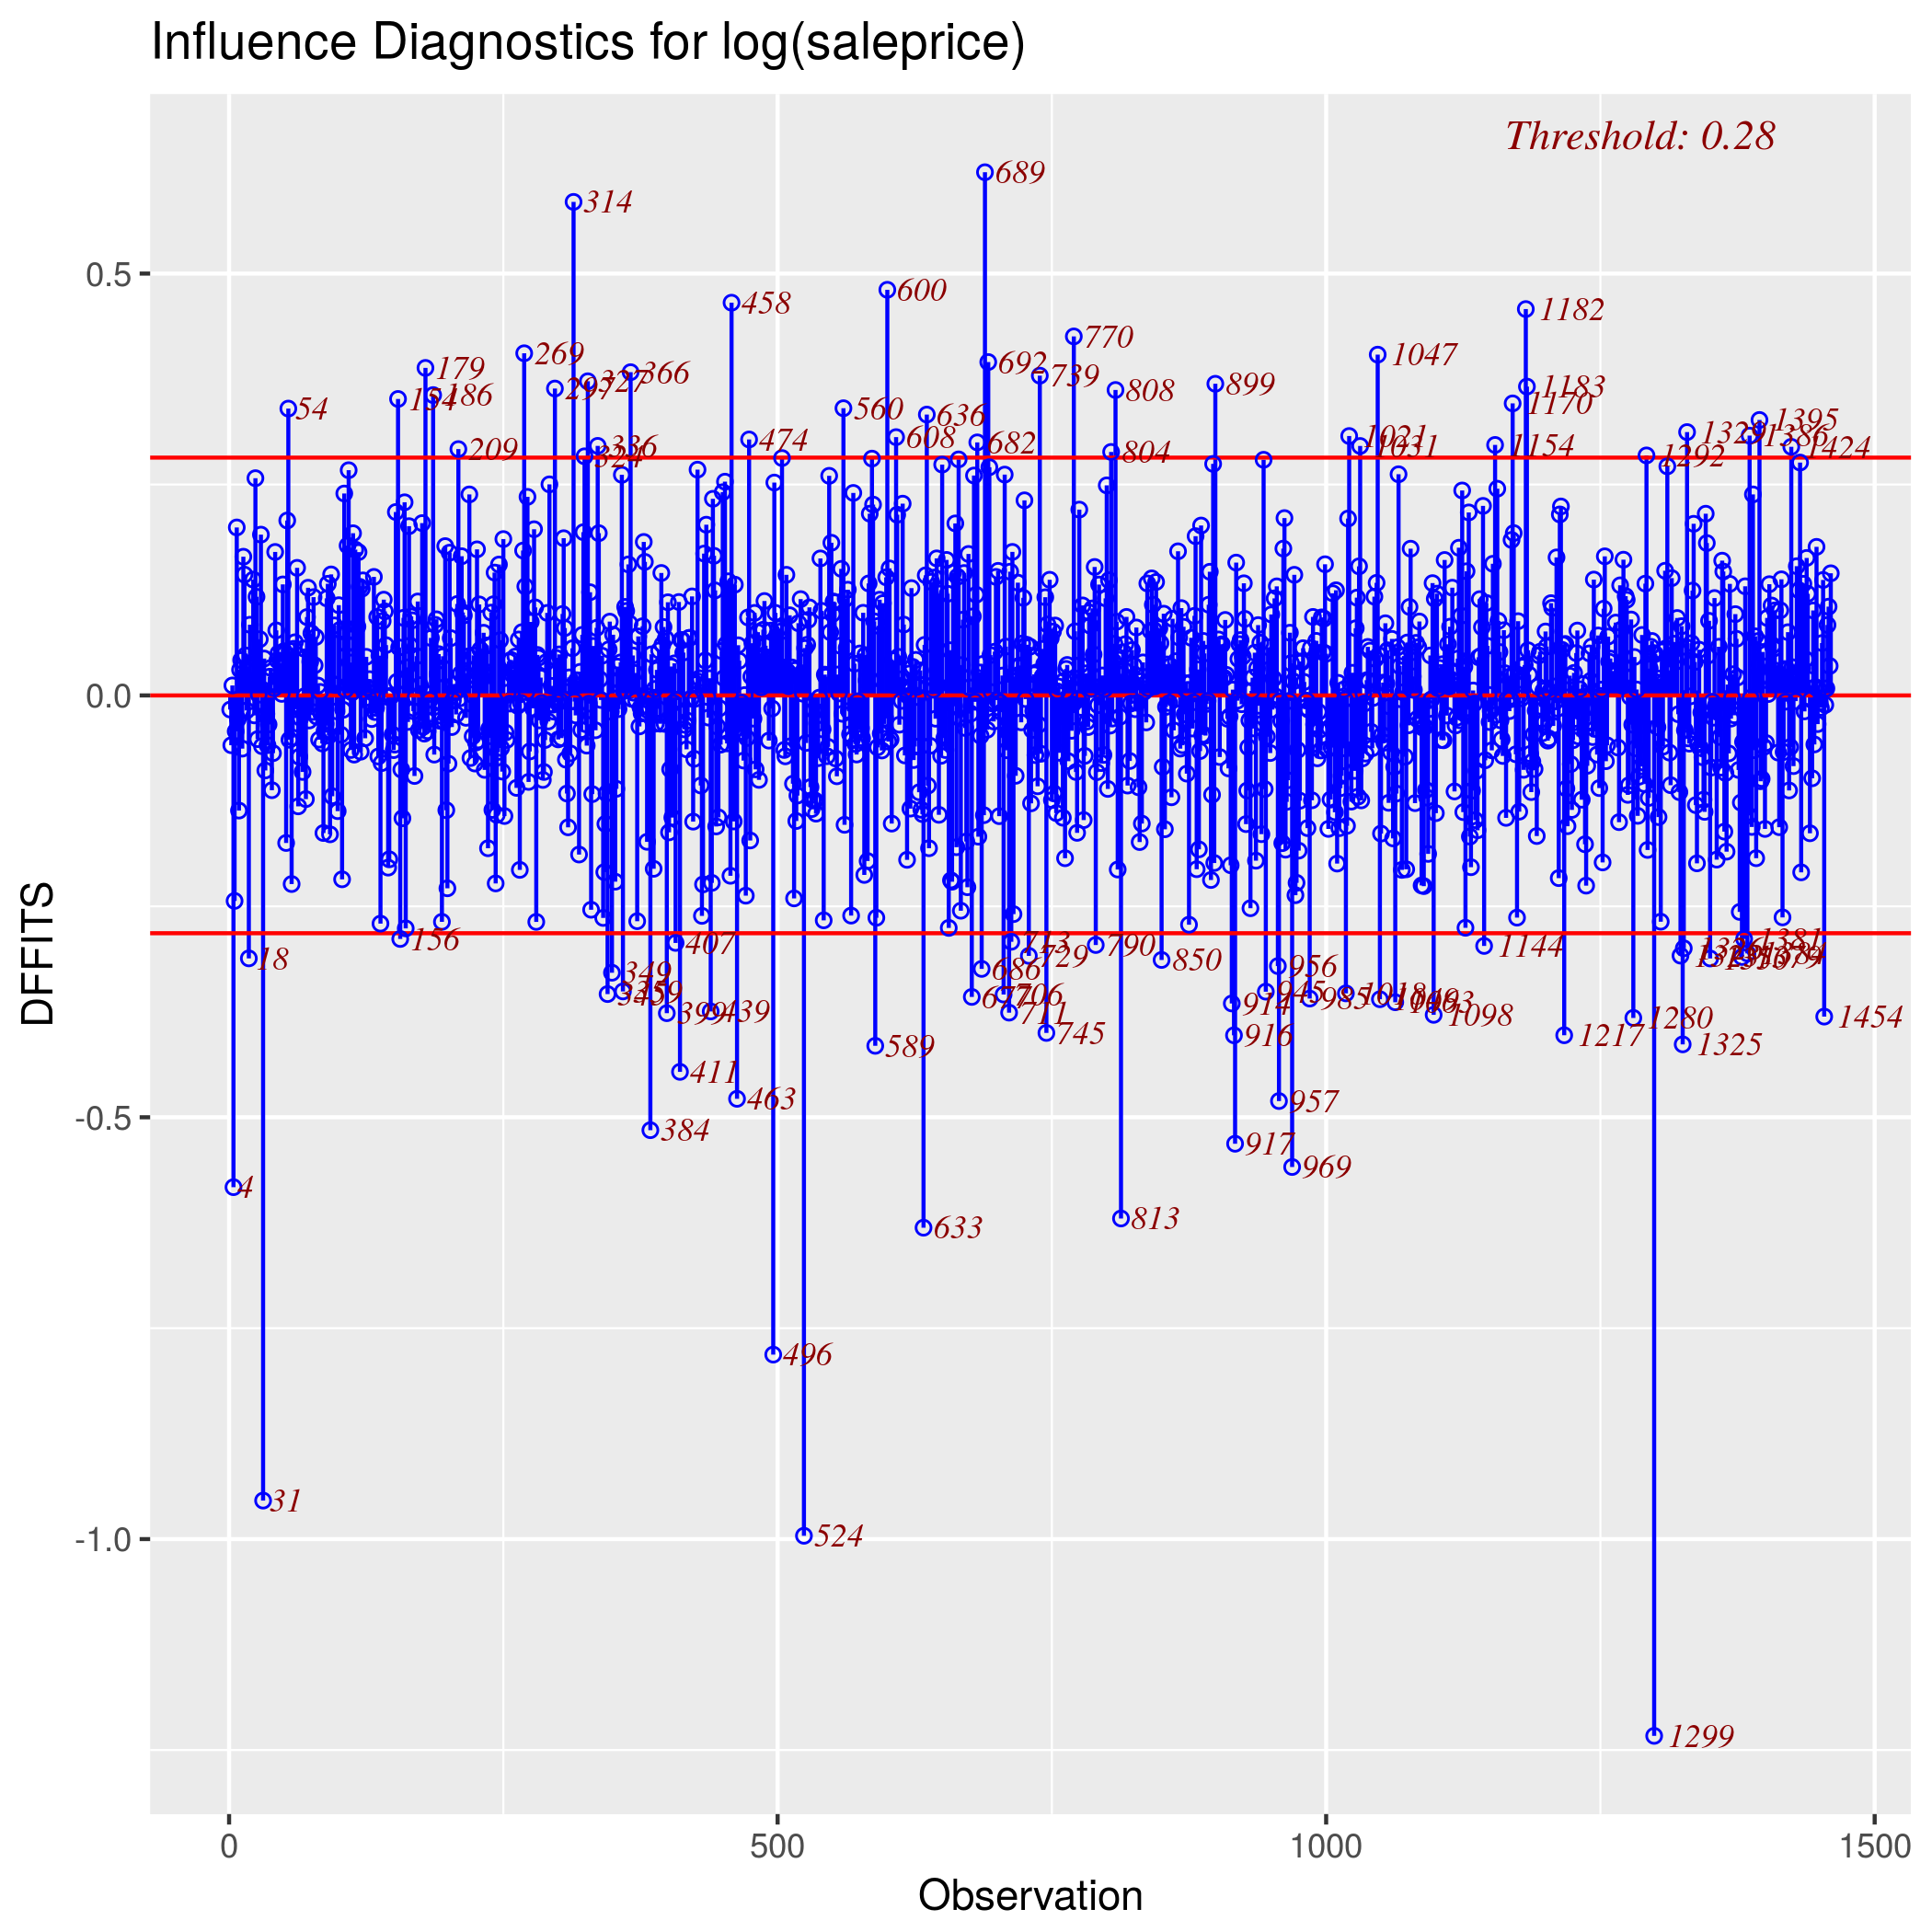
\includegraphics[scale = .5]{outlier.png}\\[1.0 cm]	

\begin{flushleft}

First, we try by removing points 1299 and 524. We see that the R squared improved slightly. If we remove \textit{all} the outliers, our R squared improved significantly. We also try to impute the outliers through with K Nearest Neighbors. The R Squared did improve but not as much as just removing. Thus, we decide to simply remove the outliers from our final model.

\end{flushleft}

\section{Visualizing Correlation}

\centering
    \vspace*{0.5 cm}
    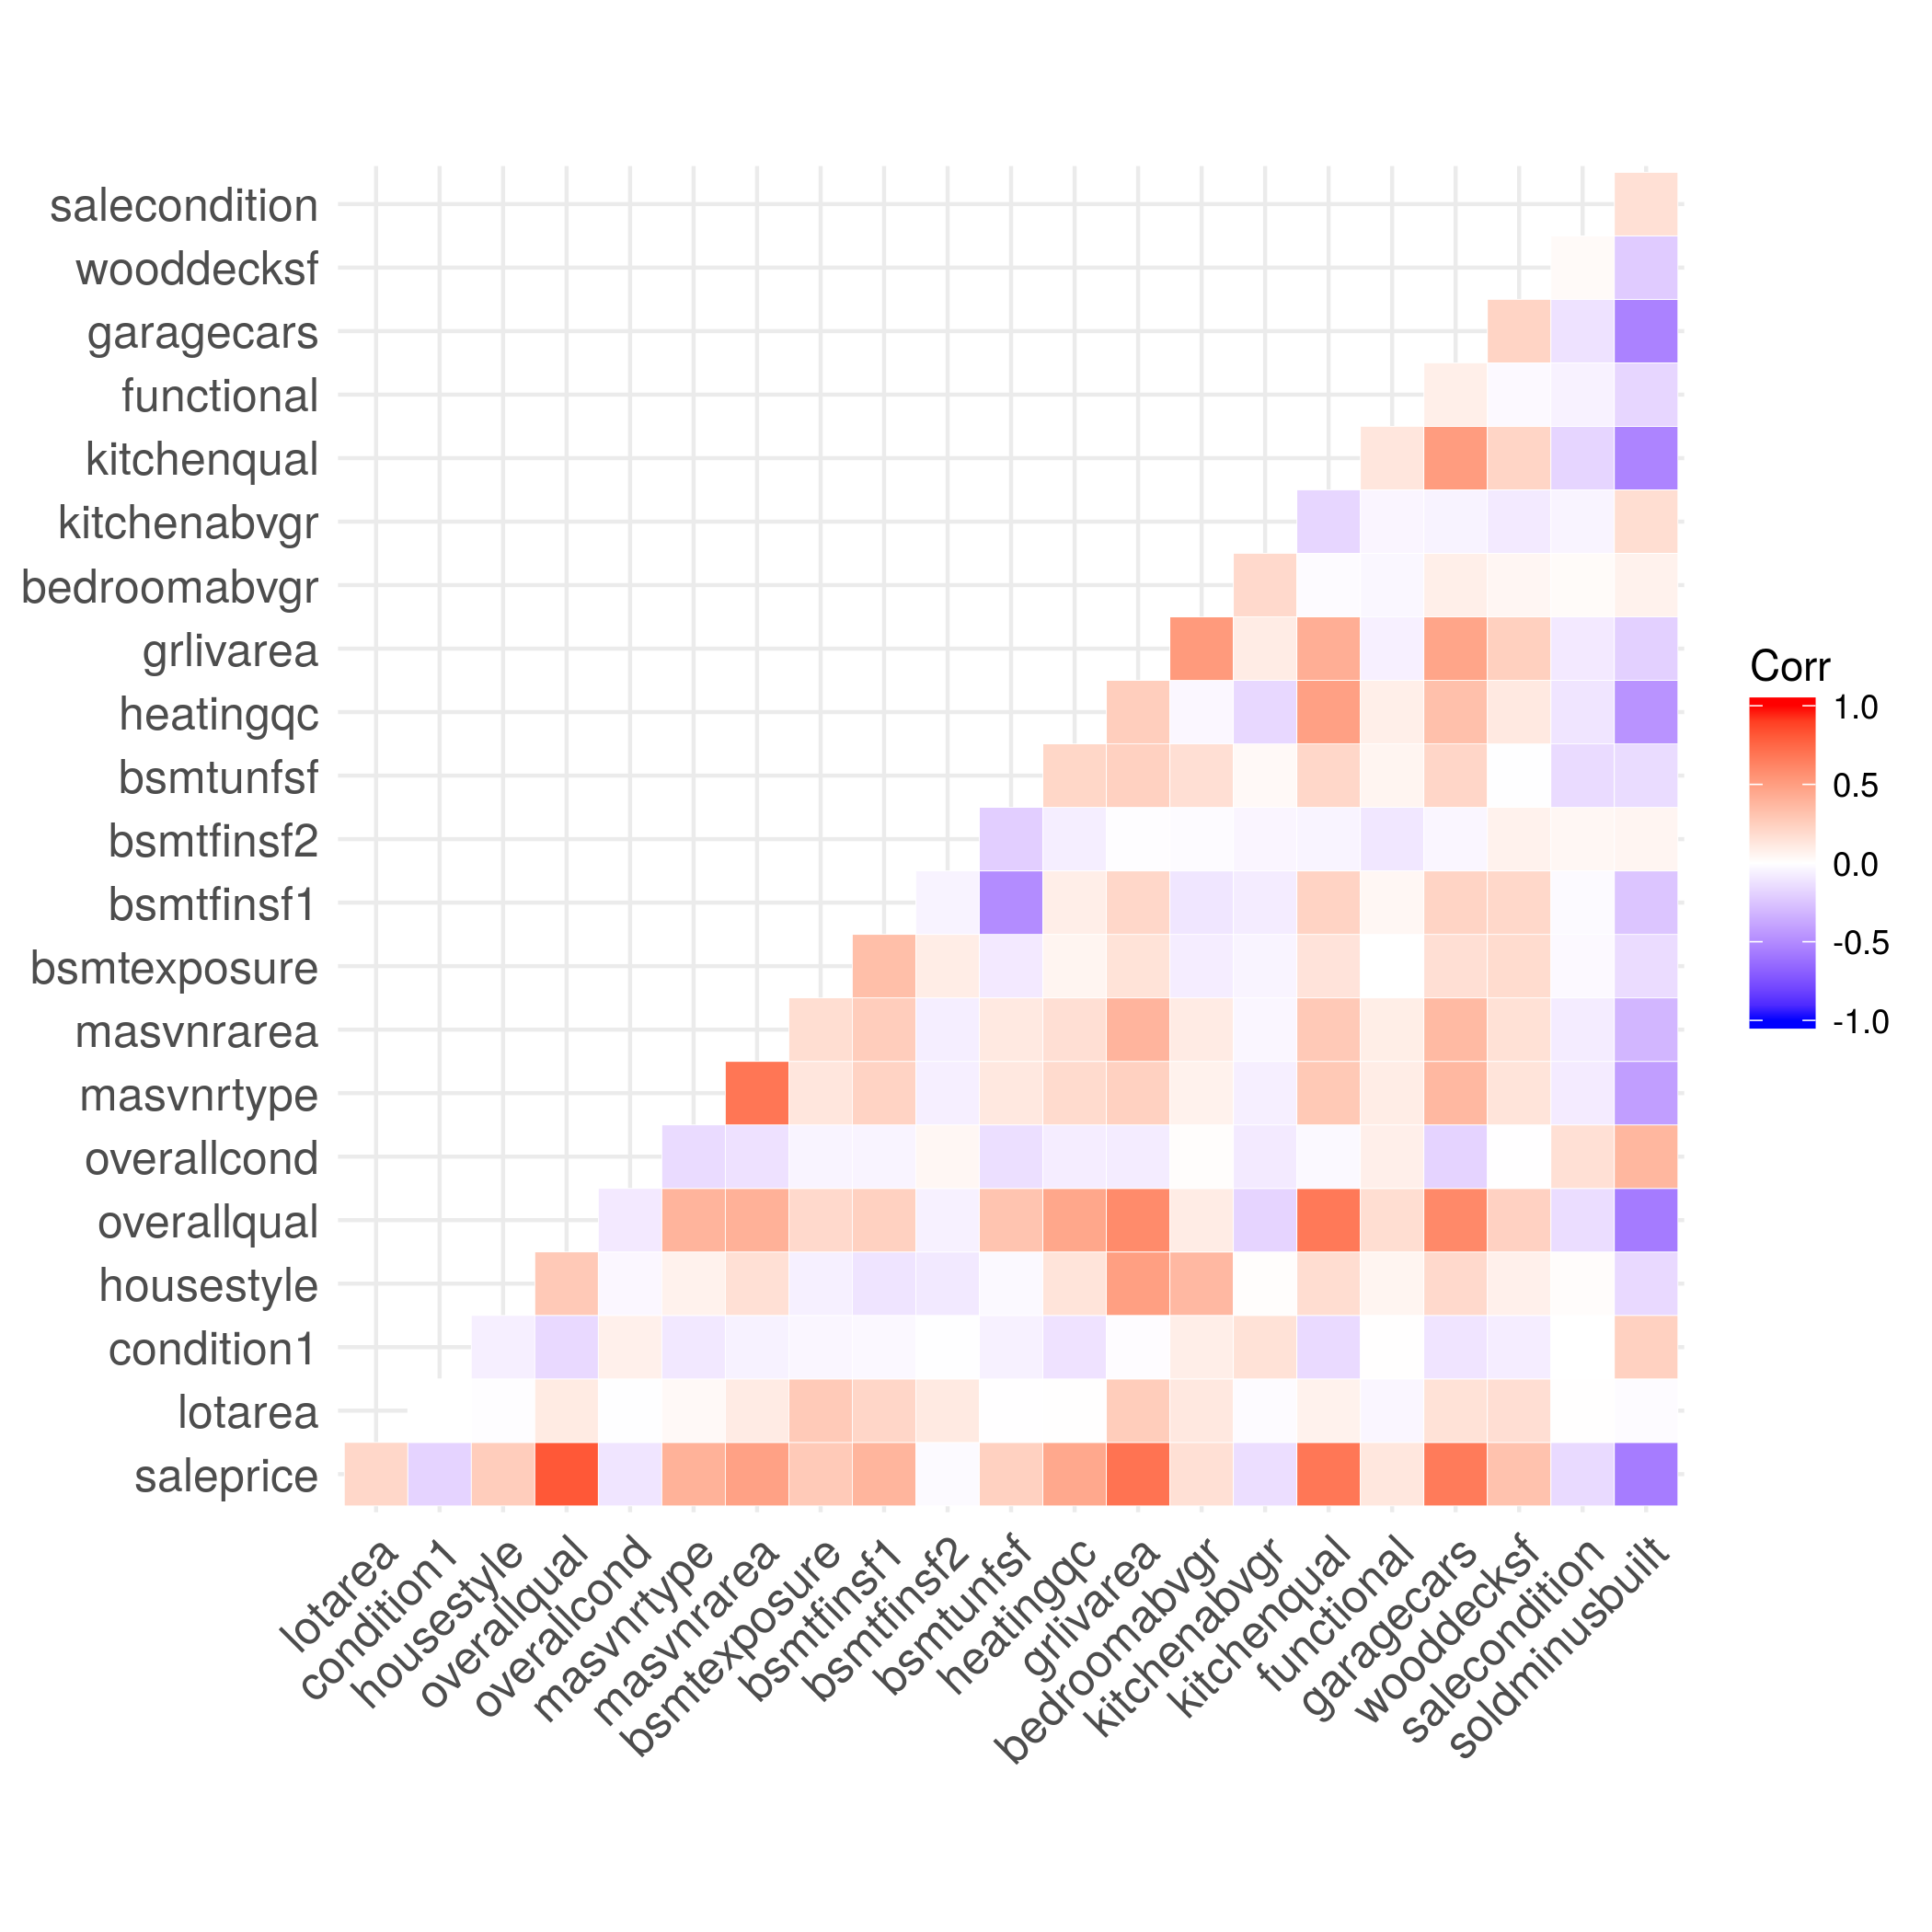
\includegraphics[scale = 1]{plot4.png}\\[1.0 cm]	
\begin{flushleft}

Looking at the bottom of the correlation plot, we see how correlated each variable is to the response variable, sale price. \textbf{In particular, the most correlated variables are overallqual, grlivarea,
kitchenqual, garagecars, and soldminusbuilt. These are the most significant predictors in predicting a house price.} With only these 5 variables in the model, they explain 83.8\% of the variation in the sale price of a house.
\end{flushleft}

\section{Valuation of Morty's House}

\begin{flushleft}

We begin our valuation of Morty's house by only selecting the 25 variables that are present in our final model. We do this by performing the function We predict the log(saleprice) then take the exponential. Computing the confidence interval we get the following: 

\centering
    \vspace*{0.5 cm}
    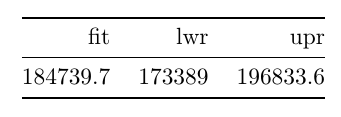
\includegraphics[scale = 0.5]{confint.png}\\[1.0 cm]	

\centering
    \vspace*{0.5 cm}
    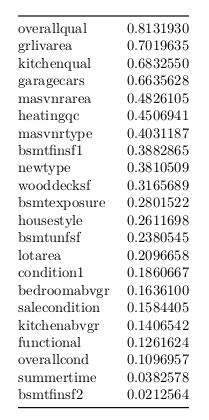
\includegraphics[scale = 0.5]{cor.png}\\[1.0 cm]	
    
\begin{flushleft}
overallqual and kitchenqual are in the top 3 for correlation with saleprice. grlivarea is difficult/nearly impossible to improve so we will move on to the next variable. Note that I removed variables like soldminusbuilt and neighborhood because they are variables that are set in stone and cannot change for obvious reasons.

Conclusion: Morty should try to improve the overallqual, which is the overall material and finish of the house. This may mean repainting some areas on the house to make it look nicer. Morty currently has a rating of 5 out 10 (average rating is 6 out of 10) so there is definitely room for improvement. Next, Morty should improve kitchenqual, which is kitchen quality. Maybe, there can be some remodeling done or fixing anything that is either old, or possibly broken. Morty has a rating of 3 out of 5 compared to the average rating of 4 out of 5. Finally, he can increase garagecars. After doing some research, it is possible to extend a garage. Although we removed garagearea since it is correlated with garagecars, both have high correlation with salesprice so Morty can consider to extend his garage -- it may be worth the investment. 

\textbf{According to our model, Morty can sell his house for a maximum value of \$ 196833.60. He should consider improving overallqual, kitchenqual, and garagecars to increase the value of his home before putting it on the market.}

\end{flushleft}



\end{flushleft}

\section{Predictive Modeling}

\begin{flushleft}

For prediction, we will try Ordinary Least Squares, Ridge regression, Lasso regression, and Elastic Net. 

\begin{flushleft}

$\lambda$ is chosen to determine whether we are performing Ridge ($\lambda = 0$ ), Lasso ($\lambda = 1$), Elastic Net ($\lambda = 0.5$). The tuning parameters in the respective models is chosen via cross validation after trying 100 different ones. The MSPE for the four models using 80$\%$ of the data for training and 20$\%$ for testing is the following:
\end{flushleft}
\centering
\begin{tabular}{ |c|c|c|c|}
\hline
OLS & 10,670,105,697 \\
Ridge & 1,769,352,685 \\
Lasso & 1,880,105,933 \\
Elastic Net & 1,875,864,966 \\
\hline
\end{tabular}
\begin{flushleft}

Our ridge model performed the best and has the lowest MSPE. This makes sense, given that our data is relatively dense, with not much zeros. Some of the "zeros" in our model are not actually zero --they are booleans that come from categorical variables that previously had 5 factors but were condensed into 2. Ridge regression helped to reduce the variation in our model, making it have the lowest MSPE.

Some variables have more impact than others but nevertheless they are statistically significant in our model so we keep them. Three of these variables are generated from other variables. We created summertime partly because of common sense and after plotting the distribution of houses being sold by month, we saw a peak in the summer months. This makes sense practically because people tend to have more time during the summer and thus are more likely to buy a house. Secondly, we created soldminusbuilt because we felt that the difference between yearsold and yearbuilt is more useful together rather than seperately. The third variable we created is a boolean for saletype to indicate a house that was "just constructed and sold", which from a common sense perspective, can make the house go much higher. Many of the variables are condensed into smaller levels. Many levels have very few observations so we feel they are not significant enough to have their own level. This helps to prevent overfitting when predicting new values. We chose to not have too many variables in our model to also prevent overfitting. We confirmed the validity of our variables through LASSO regression. Lasso didn't really eliminate any variables, which supports the statistical signifiance of our predictors. 
\end{flushleft}
\end{flushleft}

\end{flushleft}

\end{document}